\documentclass[tikz,border=8pt]{standalone}
% Shared look for every TikZ diagram. Load with \input{../../tools/tikz-style.tex}
\usepackage[T1]{fontenc}
\usepackage{lmodern}
\renewcommand{\sfdefault}{lmr}  % diagrams use the same serif as the text
\usetikzlibrary{arrows.meta, positioning, shapes.geometric, calc, fit, backgrounds}
\definecolor{cblue}{HTML}{4C78A8}
\definecolor{corange}{HTML}{F58518}
\definecolor{cgreen}{HTML}{54A24B}
\definecolor{cred}{HTML}{E45756}
\definecolor{cpurple}{HTML}{B279A2}
\definecolor{cgrey}{HTML}{6B6B6B}
\tikzset{
  every picture/.style={font=\sffamily, line width=1.2pt},
  box/.style={draw=#1, fill=#1!12, rounded corners=4pt, align=center, inner sep=7pt, minimum height=1.1cm},
  box/.default=cgrey,
  arrow/.style={-{Stealth[length=3mm]}, draw=cgrey, line width=1.4pt},
  title/.style={font=\sffamily\bfseries\Large},
  note/.style={font=\sffamily\small, text=cgrey, align=center},
}
\AtBeginDocument{\hyphenpenalty=10000 \exhyphenpenalty=10000}

% Note ML-073, Section 3: the derivation as four steps, each checked with numbers at z = 2.
% e^{-2} = 0.135, u = 1.135, sigma(2) = 0.881; both routes give 0.105 (0.13534 / 1.13534^2 = 0.88080 * 0.11920 = 0.10499).
\begin{document}
\begin{tikzpicture}[node distance=0.7cm, num/.style={font=\sffamily\large, text=cgrey, anchor=west, align=left}]
  \node[box=cblue, text width=5cm, font=\large] (a) {$\sigma(z) = \dfrac{1}{u}$, \ $u = 1 + e^{-z}$};
  \node[box=cblue, text width=5cm, font=\large, below=of a] (b) {reciprocal rule: $\dfrac{e^{-z}}{(1 + e^{-z})^2}$};
  \node[box=corange, text width=5cm, font=\large, below=of b] (c) {split: $\dfrac{1}{1 + e^{-z}} \cdot \dfrac{e^{-z}}{1 + e^{-z}}$};
  \node[box=cgreen, text width=5cm, font=\large, below=of c] (d) {$\sigma(z)\,\bigl(1 - \sigma(z)\bigr)$};
  \draw[arrow] (a) -- (b); \draw[arrow] (b) -- (c); \draw[arrow] (c) -- (d);
  \node[num] at ($(a.east) + (0.4, 0)$) {at $z = 2$: $u = 1 + 0.135 = 1.135$};
  \node[num] at ($(b.east) + (0.4, 0)$) {$0.135 / 1.135^2 = 0.105$};
  \node[num] at ($(c.east) + (0.4, 0)$) {$0.881 \times 0.119$};
  \node[num, text=cred] at ($(d.east) + (0.4, 0)$) {$= 0.105$, the same slope};
\end{tikzpicture}
\end{document}
